\section*{Metodologia}
\addcontentsline{toc}{chapter}{Metodologia}

Para resolução do problema em mãos seria necessário empregar algumas estratégias, começando pelo tratamento dos dados fornecidos no \textit{dataset}.

Inicialmente decidimos fazer o treino do modelo sem qualquer alteração ao \textit{dataset} original, simplesmente fizemos as ligações necessárias para obter um resultado.

\begin{figure}[H]
    \centering
    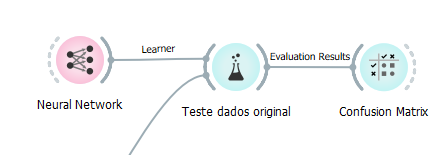
\includegraphics[]{images/testeoriginal.png}
    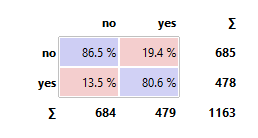
\includegraphics[]{images/confusionmatrixoriginal.png}
    \selectlanguage{portuguese} \caption{Teste \textit{Dataset} original}
\end{figure}

Conseguimos verificar que existe uma disparidade considerável na percentagem de acertos para "no" e para "yes", o que nos levou a fazer algumas verificações nos dados.

\newpage
Após uma breve verificação dos dados conseguimos chegar à conclusão que estes não se encontram simétricos, isto é, a distribuição da variável \textit{"Funded"} é superior para o caso de \textit{"no"}, isto tornaria os resultados dos modelos desequilibrados.


\begin{figure}[H]
    \centering
    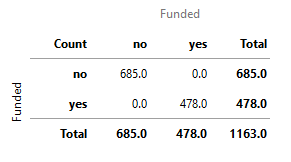
\includegraphics[]{images/pivottable.png}
    \selectlanguage{portuguese} \caption{Distribuição da variável \textit{"Funded"}}
\end{figure}

Como tal, decidimos utilizar uma amostra de 70\% dos dados de \textit{"no"}, cerca de 480, um número bastante mais próximo dos 478 dos \textit{"yes"}. Assim sendo, a amostra final não teria 1163 dados, mas sim 968 após a remoção.

\begin{figure}[H]
    \centering
    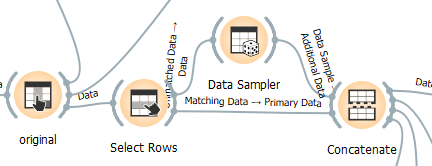
\includegraphics[scale=0.6]{images/distribuicao.png}
    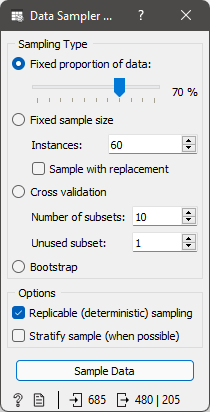
\includegraphics[scale=0.6]{images/sampleroriginal.png}
    \selectlanguage{portuguese} \caption{Distribuição dos Dados}
\end{figure}

Depois de distribuídos igualmente foi feita a normalização dos dados, para todos os valores numéricos estarem no intervalo entre [0, 1]. Foram ainda transformados todos os valores categóricos em numéricos.

Foram de seguida adicionadas duas formas de treino e teste, "Test on Train Data" e "Test on Test Data". Para o "Teste on Train Data" foram testados os dados de treino e para o "Test on Test Data" foram testados 30\% dos dados originais que foram inseridos especificamente para treino, esta divisão foi feita através de um "Data Sampler".

\begin{figure}[H]
    \centering
    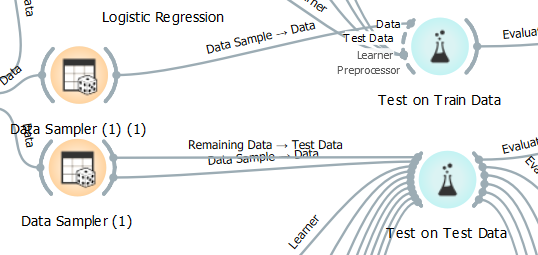
\includegraphics[scale=0.8]{images/Testetraintest.png}
    \selectlanguage{portuguese} \caption{Treino dos modelos}
\end{figure}

Os dados para o "Test on Test Data" foram divididos como 70\% dos dados para treino e os restantes para teste, já no "Test on Train Data" apenas os 70\% foram utilizados, sendo que foram usados para treino e para teste.

Foram utilizados vários tipos de modelos de aprendizagem, os modelos utilizados foram os seguintes:

\begin{itemize}
    \item Logistic Regression
    \item Neural Network
    \item Stochastic Gradient Descent
    \item Tree
    \item Random Forest
    \item Naive Bayes
    \item AdaBoost
    \item Gradient Boosting
\end{itemize}


Após obtenção dos resultados de teste dos modelos foram selecionados os Verdadeiros e Falsos Positivos e Negativos, estes foram separados e analisados através do nodo de estatística. Isto foi efetuado para verificar a existência de semelhanças entre Verdadeiros e Falsos Positivos ou Verdadeiros e Falsos Negativos.


\begin{figure}[H]
    \centering
    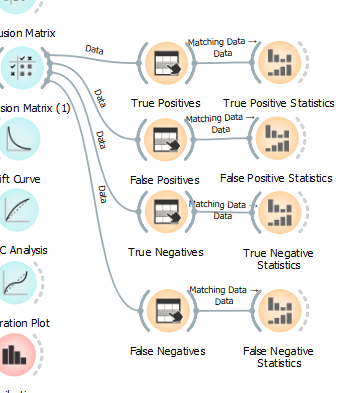
\includegraphics[scale=0.6]{images/TrueAndFalseNegativeStats.png}
    \selectlanguage{portuguese} \caption{Estatísticas dos Dados}
\end{figure}

Depois de feita a ligação comparações foram feitas entre os dados, pelo que foram encontradas algumas semelhanças em algumas variáveis.

\begin{figure}[H]
    \centering
    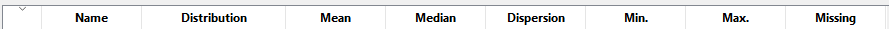
\includegraphics[scale=0.5]{images/stats.png}
    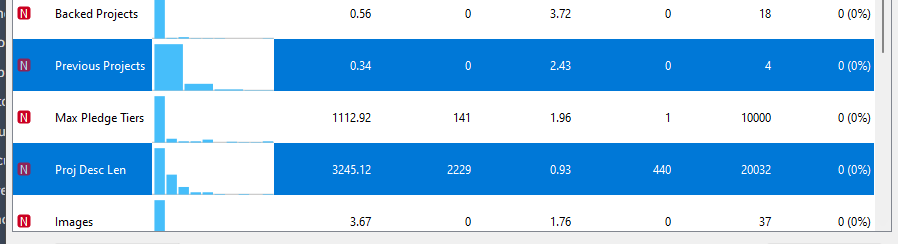
\includegraphics[scale=0.48]{images/TrueNegativeStats.png}
    \selectlanguage{portuguese} \caption{Estatísticas dos Verdadeiros Negativos}
\end{figure}

\begin{figure}[H]
    \centering
    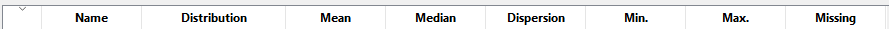
\includegraphics[scale=0.5]{images/stats.png}
    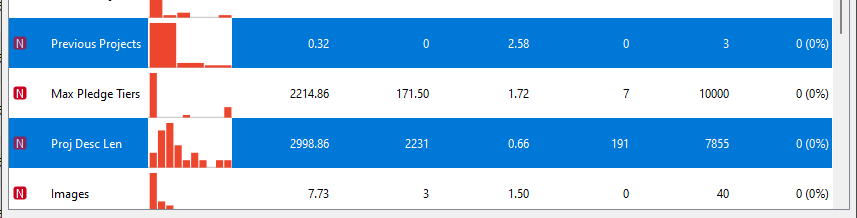
\includegraphics[scale=0.5]{images/FalseNegativeStats.png}
    \selectlanguage{portuguese} \caption{Estatísitca dos Falsos Negativos}
\end{figure}

Tanto "Previous Projects" como "Proj Desc Len" encontram-se com valores estatísticos semelhantes. Existiam outras variáveis com valores estatísticos semelhantes, pelo que todas essas variáveis foram removidas individualmente e foram verificados os resultados dos modelos para existência de alterações, pelo que foi verificado que a remoção dessas variáveis apenas afetava negativamente os resultados dos modelos.

Para finalizar o processo foram alterados os valores dos hiperparâmetros dos modelos de forma a conseguir melhores resultados.

\begin{figure}[H]
    \centering
    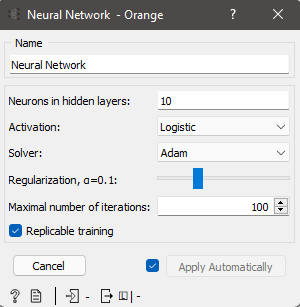
\includegraphics[scale=0.5]{images/nnhiper.png}
    \selectlanguage{portuguese} \caption{Hiperparâmetros da Rede Neural}
\end{figure}
